% !TeX spellcheck = cs_CZ
\begin{mdframed}[style=mdexam]
  \begin{example}\label{mai:exam051}
    \textbf{Grupy nemusí být tvořeny jen čísly}\newline
    Operace sčítání nebo násobení si umíme velmi dobře představit, provádíme-li je standardním
    způsobem s čísly. Definice algebraických struktur jsou však obecné a zahrnují i jiné možnosti.
    Představme si například krychli, se kterou provádíme \emph{operace symetrie}. Jsou to všechna
    taková přemístění krychle z počáteční do koncové polohy, která \uv{se nepoznají}. Znamená to, že
    krychle vypadá v koncové poloze stejně jako ve výchozí. Pokud bychom při přemísťování zavřeli
    oči, nepoznali bychom že někdo mezitím s krychlí hýbal. Přemístění jsou několikerých typů a
    definují \textbf{prvky symetrie} krychle. Abychom si je mohli názorně ukázat na obrázcích,
    označíme vrcholy, popřípadě jiné důležité body krychle písmeny. V některých ukázkách také
    použijeme hrací kostku. Prvky symetrie krychle můžeme roztřídit do následujících typů:
    \begin{itemize}
      \item \textbf{zrcadlení vzhledem k rovině symetrie} - existuje rovina, jejíž body zůstávají
            při přemístění v klidu,
      \item \textbf{rotace kolem osy symetrie} - existuje přímka (osa), jejíž body zůstávají při
            přemístění v klidu,
      \item \textbf{středová inverze} - existuje právě jeden bod (střed inverze), který při
            přemístění zůstává v klidu,
      \item \textbf{identita} - přemístění do téže polohy, v klidu jsou všechny body krychle
    \end{itemize}
    Jednotlivé typy prvků symetrie jsou znázorněny na obrázcích \ref{mai:fig037} až 4.15. Na obrázku
    \ref{mai:fig037a} jsou vyznačeny tři symetrie krychle, \(\sigma_1\), \(\sigma_2\) a
    \(\sigma_3\). Zkuste najít a nakreslit další. Druhý z obrázku 4.1. znázorňuje situaci při
    zrcadlení vzhledem k rovině \(\sigma_2\). Pro klasickou herní kostku pak operaci zrcadlení
    ilustruje obrázek 4.2.
    
    {\centering
      \captionsetup{type=figure}
      \subcaptionbox{roviny symetrie \label{mai:fig037a}}{\luafigure[0.25]{mai_fig037a.png}}
      \subcaptionbox{vzor \label{mai:fig037b}           }{\luafigure[0.25]{mai_fig037b.png}}             
      \subcaptionbox{obraz \label{mai:fig037c}          }{\luafigure[0.25]{mai_fig037c.png}}
      \captionof{figure}{Prvky symetrie krychle - zrcadlení \cite[s.~6]{Musilova2012MA2}}
      \label{mai:fig037}
    \par}

      Kolik existuje os symetrie krychle? Zkuste procvičit svou prostorovou představivost a zamyslet
      se nad touto  otázkou sami ještě dříve, než se podíváte na obrázky. Vezměte si k tomu třeba
      libovolnou hrací kostku. (Pozor, rozmístění teček na vaší kostce může být jiné, než na té
      naší, podle které jsou nakresleny obrázky.) Na obrázku 4.3 jsou vyznačeny tři osy symetrie
      \(o_1^4\), \(o_2^4\), \(o_3^4\).Prvkem symetrie je otočení kolem kterékoli z nich o jedenkrát,
      dvakrát nebo třikrát \ang{90} při čtvrtém otočeni o \ang{90} přejde krychle do původní polohy.
      Osy se proto nazývají čtyřčetné (vyznačeno horním indexem). Obrázek 4.4 znázorňuje konkrétní
      situaci při otočení o úhel \ang{270} kolem osy o, zatímco obrázek 4.5 ukazuje toto otočení pro
      klasickou herní kostku.

    {\centering
      \captionsetup{type=figure}
      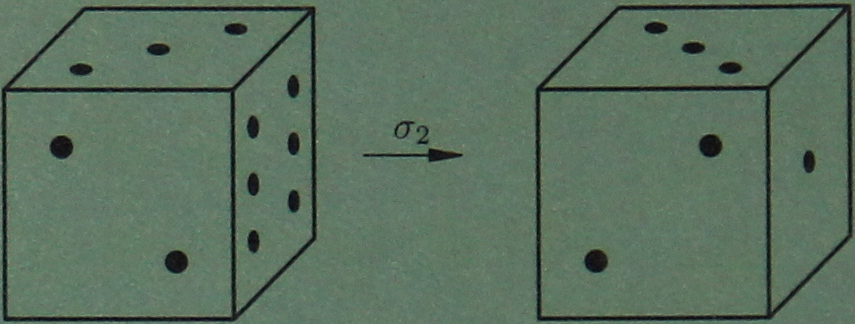
\includegraphics[width=0.4\linewidth]{mai_fig038.png}
      \captionof{figure}{Prvky symetrie hrací kostky - zrcadlení. \cite[s.~7]{Musilova2012MA2}
      \label{mai:fig038}}
      \par}
    
      Další čtyři osy symetrie odpovídají tělesovým úhlopříčkám krychle a jsou znázorněny na obrázku
      4.6. Jsou označeny symboly \(o_1^3\), \(o_2^3\), \(o_3^3\) a \(o_4^3\) a nazývají se trojčetné
      (víte proč?).

    {\centering
      \captionsetup{type=figure}
      \subcaptionbox{možné osy \label{mai:fig039a}}{\luafigure[0.25]{mai_fig037a.png}}
      \subcaptionbox{vzor \label{mai:fig039b}     }{\luafigure[0.25]{mai_fig037b.png}}
      \subcaptionbox{obraz \label{mai:fig039c}    }{\luafigure[0.25]{mai_fig037c.png}}
      \captionof{figure}{Prvky symetrie krychle - zrcadlení \cite[s.~6]{Musilova2012MA2}}
      \label{mai:fig039}
    \par}


      Obrázky 4.7 a 4.8 odpovídají konkrétnímu otočení kolem osy \(o_3^3\) o úhel \ang{270}.

    {\centering
      \captionsetup{type=figure}
      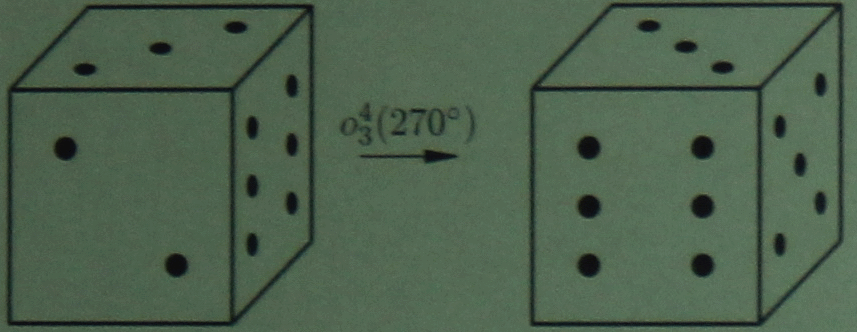
\includegraphics[width=0.4\linewidth]{mai_fig040.png}
      \captionof{figure}{Prvky symetrie krychle - otáčení. \cite[s.~8]{Musilova2012MA2}
      \label{mai:fig040}}
      \par}
      

    {\centering
      \captionsetup{type=figure}
      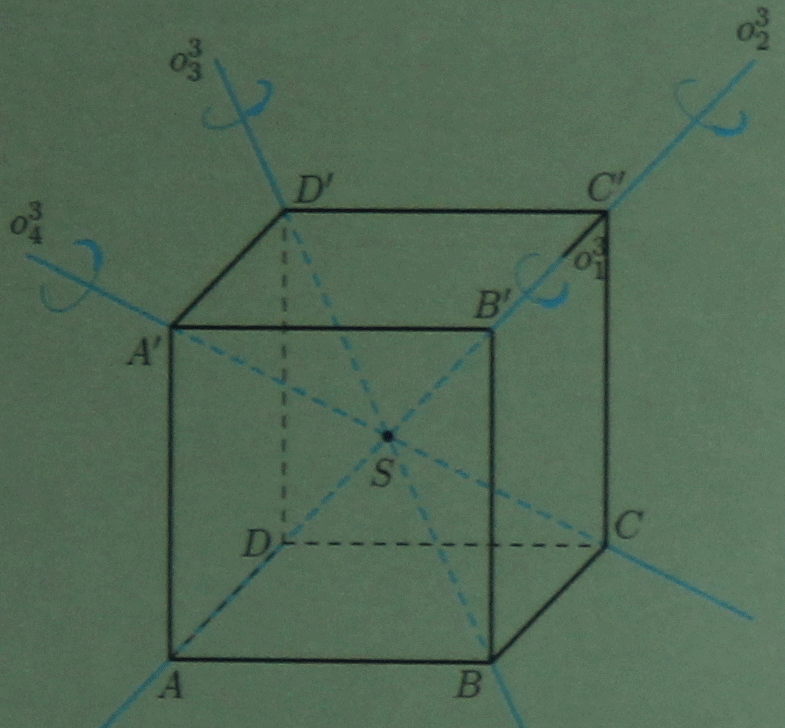
\includegraphics[width=0.4\linewidth]{mai_fig041.png}
      \captionof{figure}{Prvky symetrie krychle - otáčení. \cite[s.~8]{Musilova2012MA2}
      \label{mai:fig041}}
      \par}

    {\centering
      \captionsetup{type=figure}
      \subcaptionbox{vzor \label{mai:fig042a} }{\luafigure[0.25]{mai_fig042a.png}}
      \subcaptionbox{obraz \label{mai:fig042b}}{\luafigure[0.25]{mai_fig042b.png}}
      \captionof{figure}{Prvky symetrie krychle - zrcadlení \cite[s.~9]{Musilova2012MA2}}
      \label{mai:fig042}
    \par}

    {\centering
      \captionsetup{type=figure}
      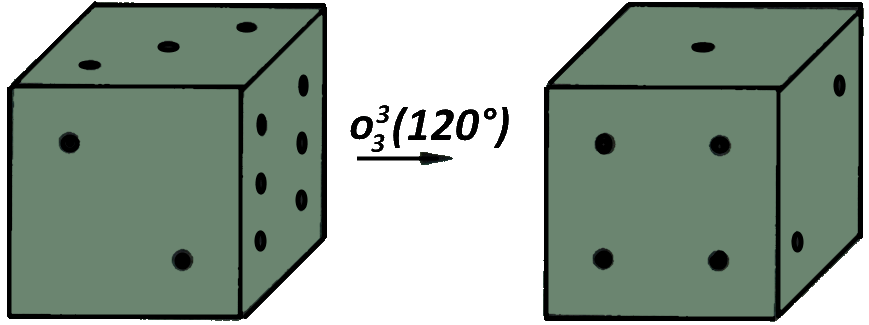
\includegraphics[width=0.4\linewidth]{mai_fig043.png}
      \captionof{figure}{Prvky symetrie krychle - otáčení. \cite[s.~9]{Musilova2012MA2}
      \label{mai:fig043}}
      \par}

      Dalších šest os symetrie najdeme v obrázku 4.9. Každá z nich vždy prochází bodem S (průsečíkem
      tělesových úhlopříček) a spojuje středy protilehlých hran. Tyto dvojčetné osy jsou označeny
      symboly \(o_1^2\), \(o_2^2\), \(o_3^2\), \(o_4^2\), \(o_5^2\), \(o_6^2\). Konkrétní příklad
      otočení kolem osy \(o_1^2\) o úhel \qty{180}{\degree} ilustrují obrázky 4.10 a 4.11. Obrázky
      4.12 a 4.13 znázorňují středovou inverzi a obrázky 4.14 a 4.15 identitu.
      
      Přemístění můžeme \textbf{skládat}, tzn. postupně provádět . Polohy, ve kterých (neoznačená)
      krychle vypadá stejné, nazveme ekvivalentní. Označme \(A\) určitou polohu krychle a
      \(\mathcal{P}_A\) množinu všech přemístění krychle mezi kteroukoli dvojici poloh
      ekvivalentních poloze \(A\). Operaci skládání přemístění definujeme takto: Nechť
      \(\varrho\ni\mathcal{P}_A\) je přemístění krychle z polohy \(B\) do polohy \(C\) a
      \(\psi\ni\mathcal{P}_A\) její přemístění z polohy \(C\) do polohy \(D\). Označme jako
      \(\psi\circ\varrho\) přemístění,které vznikne postupným provedením nejprve \(\varphi\) a potom
      \(\psi\). Vzniká tak zobrazení
      \begin{equation*}
        \mathcal{P}_A\times\mathcal{P}_A\ni [\varphi,\psi] 
          \longrightarrow\psi\circ\varphi\in\mathcal{P}_A,
      \end{equation*}
      která je typu (\ref{mai:eq047}). Asociativní zákon (\ref{mai:eq048}) je splněn, identita
      (přesunutí do téže polohy) je neutrálním prvkem, zpětné přemístění z polohy \(C\) do \(B\) je
      inverzním prvkem k přemístění \(\varphi\). Množina \(\mathcal{P}_A\) s operací skládání
      přemístění je grupou. Není však grupou komutativní, jak ukazují obrázky (4.16, 4.17 a 4.18).
      Tato grupa má velmi zajímavé vlastnosti. Na rozdíl od všech předchozích příkladů grup je počet
      jejich prvků konečný. Navíc každá z prvků symetrie krychle definuje jistou podgrupu grupy
      \(\mathcal{P}_A\). Vezměme například trojčetnou osu symetrie \(o_3^3\) zadanou tělesovou
      úhlopříčkou \(BD'\) na obrázcích 4.6 a 4.7. Přemístění, která s touto osou souvisejí, jsou
      všechny rotace kolem ní o úhel, který je celistvým násobkem úhlu \ang{120}. Patří sem i
      identita, \(\mathcal{P}_A\). Všimněme si, že každý prvek této podgrupy můžeme dostat pomocí
      skládání jediného prvku sama se sebou. Tímto jediným prvkem je rotace kolem osy \(o_3^3\) o
      úhel \ang{120}. Grupa s takovou vlastností se nazývá \textbf{cyklická}. Zkuste zjistit, které
      další cyklické podgrupy obsahuje grupa operací symetrie krychle. 
      
      Pozn.: Obecně se grupa \(G\) nazývá cyklická, jestliže je tvaru
      \begin{equation*}
        G = \{a, a^2 \ldots a^{n-1}, a^n = e_G\}.
      \end{equation*}
      Číslo \(n\) je rovno řádu grupy. Cyklické grupy se významně uplatní například v
      krystalografii.
      
      A uvědomme si ještě, o co zajímavější ale složitější, by naše úvahy byly, kdybychom se
      zajímali o grupu operací symetrie\textbf{ Rubikovy kostky}! 
  \end{example}
\end{mdframed}